\documentclass{BeamerTemplate}

\title{Module 9 - Analyse de la variance à un facteur}

\graphicspath{{Images/Module 9/}}

\begin{document}
\begin{frame}[t]
  \titlepage
\end{frame}

%-------------------------------------------------------------------------------------------------------------------------------------


    


%%%%%%%%%%%%%%%%%%%%%%%%%%%%%%%%%%%
%%%%%%%%%%%%%%%%%%%%%%%%%%%%%%%%%%%
%%%%%%%%%%%%%%%%%%%%%%%%%%%%%%%%%%%

%\section[Intro]{Introduction}
\section[Principes]{Principes d'expérimentation}
\subsection*{ }


\begin{frame}[t]
 \frametitle{Principes d'expérimentation}

 {\small
 Pour qu'une expérience mène à une découverte réelle,
 \begin{enumerate}\itemsep0mm
 %\item L'expérimentation est à la base de toute découverte.
 \item  l'expérience doit  être bien planifiée,
 \item les résultats doivent être adéquatement analysés.
\end{enumerate}

\medskip
\uncover<2->{
Pourquoi planifier une expérience?
\begin{itemize}\itemsep0mm
\item se protéger contre les sources de biais potentielles,
\item contrôler la variabilité due à certains facteurs.
\end{itemize}
}
}
\end{frame}

\begin{frame}[t] \frametitle{Une expérience sur la durabilité des batteries}


\small

But: Déterminer quel type de batterie (Lithium-ion, Lithium-fer-phosphate ou Nickel-hydrure métallique) conserve le mieux sa capacité après 500 cycles de recharge.\\[2mm]

Plusieurs variables influentes:

     \begin{itemize}
    \item Le chargeur utilisé peut légèrement varier d’une station à l’autre. %On dispose de 4 fusils.
    \item La température ambiante dans la salle d’essai n’est pas parfaitement stable.
    \item Les capteurs de mesure de capacité ont de légers biais entre les bancs de test.
    %\item On dispose d'un nombre limité d'unités à peinturer puis à faire cuire.
\end{itemize}


Comment concevoir l’expérience pour isoler l’effet du type de batterie malgré les variations causées par les chargeurs, les conditions ambiantes et les instruments de mesure ?


\end{frame}

% image: http://www.caneo-france.fr/peinture-industrielle/
%image 2: http://www.peintureomax.com/fr/

\begin{frame}[t]
 \frametitle{Principes d'expérimentation}

Trois principes essentiels:\\[2mm]

\begin{itemize}\itemsep7mm
\item identification des sources de variabilité (pour les contrôler).
\item répétition (pour estimer la variabilité)
\item randomisation (pour éliminer les biais)
\end{itemize}
\end{frame}

\begin{frame}[t]
 \frametitle{L'analyse de la variance}

\alert{L'analyse de la variance}  compare l'effet des sources de variabilité. Utile pour:


%Une fois une expérience terminée, il faut en analyser les résultats pour
\begin{itemize}\itemsep2mm
\item déterminer si les différences observées sont bien dues aux facteurs d'intérêt et non à la chance
\item construire un modèle de prévision
\item déterminer la combinaison optimale des facteurs
\end{itemize}
%Pour ce faire, on a recours aux techniques dites d'

\medskip
On dit  \alert{anova}, pour {\it \underline{AN}alysis \underline{O}f \underline{VA}riance}.
\end{frame}


\section[Plan 1 facteur]{Plan d'expérience à un facteur}\label{sec:1fac}

\subsection{Contexte et vocabulaire}

\begin{frame}[t]{But d'une expérience à un facteur}
\underline{Comparer 2 moyennes}:\\
%On sait tester, à partir de 2 échantillons indépendants, si les moyennes de 2 populations normales de même variance sont égales  ($H_0:  \mu_1=\mu_2$, cas 2).
$\left.\begin{array}{l}
\text{2 populations normales }\\
\text{variances égales}\\
H_0:  \mu_1=\mu_2
\end{array}\right\} \text{test } t \text{ à 2 échantillons indépendants}$

\bigskip
\uncover<2->{
\underline{\alert{Comparer plusieurs moyennes}}:\\
%Comment tester  \alert{si les moyennes de plusieurs populations sont égales}?

$\left.\begin{array}{l}
a \text{ populations normales }\\
\text{variances égales}\\
\begin{array}{ll}
H_0:& \mu_1=\mu_2=...=\mu_a\\
H_1:& \mu_k\ne\mu_l\;\text{ pour au moins }  \\
&\qquad\qquad\text{ une paire } (k,l) \
\end{array}
\end{array}\right\} \begin{array}{c}\text{analyse de la variance}\\
\text{à 1 facteur}\\ (a \text{ échantillons indépendants})\end{array}$



\bigskip
\alert{On veut tester l'effet d'un facteur sur la moyenne d'une variable.}

}
\end{frame}



\begin{frame}[t]{Vocabulaire}

\begin{itemize}\itemsep2mm
    \item<1-> \alert{Variable réponse}: La variable pour laquelle nous désirons tester l'égalité des moyennes. Appelée  aussi \textit{variable dépendante}, notée $Y$.
    \item<2-> \alert{Facteur}: Ce qui différencie les populations ou les traitements. 
    Chaque traitement ou population correspond à un \textit{niveau} du facteur, ou à une \textit{modalité} du facteur.
    \item<3-> \alert{Unités expérimentales}: Les individus ou objets sur lesquels le traitement est appliqué.
\end{itemize}

\vspace{5mm}

%Notons que les golfeurs sont indépendants, mais pas les mesures que l'on prend sur un même golfeur.
\uncover<3->{En anova à un facteur, \alert{les échantillons doivent être indépendants} (une seule mesure par unité expérimentale).}

\end{frame}



\begin{frame}[t]{ }

\centerline{\LARGE\bf \alert{QUIZ !}}
\bigskip

Dans l'expérience sur les batteries, identifiez les quantités suivantes:
\bigskip

\begin{enumerate}[$\bullet$]\itemsep 7mm
\item La variable réponse % Temps de séchage
\item Le facteur et le nombre de niveaux % Type de peinture
\item L'unité expérimentale %pièce peinte
\end{enumerate}

\vspace{6mm}

\end{frame}

\subsection{Devis d'expérience et données}

\begin{frame}[t]{Devis de l'expérience à un facteur}

{\small
%On veut mesurer \alert{l'effet d'un facteur à $a$ niveaux  sur la valeur moyenne d'une variable réponse} donnée.

Deux scénarios d'échantillonnage possibles:%Le plan d'expérience à un facteur consiste à mener l'un de ces deux types d'expérience:
\begin{enumerate}
\item<1-> Choisir $n\times a$ unités expérimentales. Déterminer aléatoirement\\
$n$ unités qui recevront le traitement $1$, \\
$n$ unités qui recevront le traitement $2$, \\...,\\
$n$ unités qui recevront le traitement $a$;
\item<2-> échantillonner aléatoirement $n$ unités dans la population $1$,\\
échantillonner aléatoirement $n$ unités dans la population $2$, \\...,\\
échantillonner aléatoirement $n$ unités dans la population $a$.
\end{enumerate}

\uncover<3->{
Dans les deux cas, on obtient \alert{$a$ échantillons indépendants de taille $n$ }.\\
$\Rightarrow$ on obtient les observations $$Y_{ij},\quad\text{où }
\begin{array}{l} i=1,\ldots,a,\\ j=1,\ldots,n.
\end{array}$$
}
}
\end{frame}
\begin{frame}[t]{Notation pour les sommes et moyennes}
Le symbole $\bullet$ signifie qu'une moyenne ou une somme est calculée pour \alert{toutes les valeurs de l'indice que $\bullet$ remplace}.

\medskip
{\small
Supposons $y_{ij}$ pour $i=1,\ldots,6$, $j=1,\ldots,8$. On aurait, par exemple,
\begin{align*}
y_{\bullet j}&=\sum_{i=1}^6y_{ij}\\
\overline{y}_{i\bullet }&=\frac{1}{8}\sum_{j=1}^8y_{ij}\\
y_{\bullet\bullet}&=\sum_{i=1}^6\sum_{j=1}^8y_{ij}\\
\overline{y}_{\bullet \bullet}&=\frac{1}{6\times 8}\sum_{i=1}^6\sum_{j=1}^8y_{ij}
\end{align*}

}
\end{frame}
% Source image: http://www.das-europe.com/wastewater-treatment-textile-industry.html
\begin{frame}[t]{Exemple 1:  la force du textile}

Un ingénieur veut savoir si la force de résistance  d'une fibre textile est différente selon la proportion de coton dans la fibre.
\medskip

Son expérience : mesurer la résistance pour 25 unités de tissu fabriquées avec différentes proportions de coton.

\bigskip


\medskip
\end{frame}
\begin{frame}[t]{Exemple 1: les données (en {\it psi}, lbs/pouce carré)}

{\small
\begin{tabular}{c|ccccc|ccc}\hline
Pourcentage & \multicolumn{5}{c|}{Observations $j$} & Somme & Moy.& É.-type\\
de coton $i$ & 1 & 2 & 3 & 4 & 5 & $y_{i\bullet}$ & $\overline{y}_{i\bullet}$ & $s_i$\\ \hline
15 & 7 & 7 & 15 & 11 & 9 & 49 & 9,8 &3,35\\[2mm]
20 & 12 & 17 & 12 & 18 & 18 & 77 & 15,4 &3,13\\[2mm]
25 & 14 & 18 & 18 & 19 & 19 & 88 & 17,6&2,07 \\[2mm]
30 & 19 & 25 & 22 & 19 & 23 & 108 & 21,6&2,61 \\[2mm]
35 & 7 & 10 & 11 & 15 & 11 & 54 & 10,8 &2,86\\ \hline
&&&&&&\multicolumn{2}{r}{$\overline{y}_{\bullet\bullet}=15,04$}
\end{tabular}
}

\vspace{2.7cm}
{\tiny Source: {\it Design and Analysis of Experiments}, D.C. Montgomery (2001).}
\end{frame}

\begin{frame}[t]{Exemple 1: représentation graphique}
\begin{center}
\begin{tikzpicture}
  \begin{axis}[
    xlabel={Pourcentage de coton},
    ylabel={Résistance du tissu},
    xmin=12, xmax=38,
    ymin=6, ymax=27,
    width=10cm,
    height=8cm,
    only marks,
    mark=*,
    tick label style={font=\small},
    grid=none
  ]

  % Points extraits du graphique
  \addplot[color=black, mark=*] coordinates {
    (15,7) (15,15) (15, 11) (15, 9)
    (20,12) (20,17) (20,18)
    (25,14) (25,18) (25,19)
    (30, 19) (30,22) (30,23) (30,25)
    (35,7) (35,10) (35,11) (35, 15)
  };

  \end{axis}
\end{tikzpicture}
\end{center}
\end{frame}

\subsection[Modèle]{Modèle et postulats}


\begin{comment}
\begin{frame}[t]{Autre formulation du modèle}
Comme les \alert{différences entre les moyennes des traitements} nous intéressent plus que les moyennes
elles-mêmes, il est d'usage de récrire le modèle ainsi:
$$
Y_{ij}=\alert{\mu+\tau_i}+E_{ij},\ \ \ i=1,\ldots,a,\ \ j=1,\ldots,n,
$$
où l'on décompose $\mu_i$ (la moyenne de la population $i$) en une
moyenne globale, $\mu$, et la différence entre la moyenne
de la population $i$ et la moyenne globale, $\tau_i$:
$$\mu_i=\mu+(\mu_i-\mu)=\mu+\tau_i,$$
où $\tau_i=\mu_i-\mu$.
\end{frame}

\begin{frame}[t]{Contrainte sur les valeurs des $\tau_i$}
Pour que $\mu$ soit bien la moyenne des $\mu_i$, on
doit avoir
\begin{align*}
\mu&=\frac{1}{a}\sum_{i=1}^a\mu_i=\frac{1}{a}\sum_{i=1}^a(\mu+\tau_i)\\
&=\frac{1}{a}(a\mu+\sum_{i=1}^a\tau_i)=\mu+\frac{1}{a}\sum_{i=1}^a\tau_i\\
\Leftrightarrow \sum_{i=1}^a\tau_i&=a(\mu-\mu)=0.
\end{align*}
\end{frame}
\end{comment}
\begin{frame}[t]{Modèle et interprétation}

{\small
$$\begin{array}{lcccl}
Y_{ij} & = & \alert{\mu_i} &+& E_{ij},\qquad\textrm{où}~~~i=1, \ldots, a,~~j=1, \ldots, n,
\\[0.3cm]
 & = & \alert{\mu + \tau_i} &+& E_{ij},%~~~\textrm{où}~~~i=1, \ldots, a,~~j=1, \ldots, n_i,
\end{array}$$

où
\begin{itemize}
\item<1->[$Y_{ij}$]:  valeur de la variable réponse pour l'observation $j$ de l'échantillon/du traitement $i$;
\item<2->[$\mu_i$]:  valeur moyenne de $Y$ dans la population $i$ ;
\item<3->[$\mu$]:  moyenne  globale de $Y$ (toutes pop. confondues);
\item<4->[$\tau_i$]:  différence entre la moyenne du traitement $i$ et la moyenne globale ($\tau_i=\mu_i-\mu$). %On l'appelle  {\em effet du $i$-ème traitement} et
    On a la contrainte $\sum_{i=1}^a\tau_i=0$;
\item<5->[$E_{ij}$]:  terme d'erreur pour la $j^e$ observation du traitement $i$;
\end{itemize}
\uncover<5->{
\href{https://jmiron-anovapara.share.connect.posit.cloud/}{Illustration des paramètres}}}

\end{frame}


\begin{frame}[t]{Postulats du modèle}
%Afin de pouvoir estimer l'effet des traitements et de tester si le facteur est significatif de fa\c{c}on formelle, nous nous baserons sur les postulats suivants:
Le modèle se base sur les postulats suivants:

\begin{itemize}
\item[(P1)] Les $a$ échantillons sont indépendants.
\item[(P2)] La variance des $Y_{ij}$ est homogène entre les traitements.
\item[(P3)] Les $Y_{ij}$ sont des variables indépendantes de loi normale.
\end{itemize}

\medskip
\uncover<2->{
Nous pouvons résumer ces  postulats ainsi:
$$
Y_{ij}=\mu_i+E_{ij},\quad \ \ % i=1,\ldots,a,\ \ j=1,\ldots,n,
\text{ où }\; \alert{E_{ij}\;\text{ sont des v.a. i.i.d. }\;N(0,\sigma^2)}.
$$

Ces postulats devront être vérifiés avant de tirer des conclusions basées sur des tests d'hypothèses.}
\end{frame}


\section[Inférence globale]{Estimation et test d'hypothèses}\label{sec:infe1fac}
\subsection*{ }

\begin{frame}[t]{Estimation ponctuelle des paramètres}

{\small
\begin{itemize}
\item<1-> Paramètres inconnus du modèle : $\mu,\tau_1,\ldots,\tau_a$ et $\sigma^2$.
\item<2-> L'estimateur de $\mu$ est \alert{$\hat{\mu}=\overline{y}_{\bullet\bullet}$}, la moyenne de toutes les observations.
\item<3-> On estime $\mu_i$ par la moyenne des observations du traitement $i$, \alert{$\hat{\mu}_i=\overline{y}_{i\bullet}$}.
\item<4-> Puisque $\tau_i=\mu_i-\mu$, on a que \alert{$\hat{\tau}_i=\overline{y}_{i\bullet}-\overline{y}_{\bullet\bullet}$}.
\item<5-> La variance étant considérée égale dans tous les traitements, on estime $\sigma^2$ en combinant les variances des $a$ échantillons: \alert{$\hat{\sigma}^2=\dfrac{S_1^2+...+S_a^2}{a}=MS_E$}.
\end{itemize}
}

\end{frame}

\begin{frame}[t]{Exemple 1}
Quelles sont les estimations des paramètres pour l'exemple 1? \href{https://jmiron-anovapara.share.connect.posit.cloud/}{Illustration}
\end{frame}


\begin{frame}[t]{Les hypothèses testées}
La question la plus importante dans ce type d'étude est\\
 \centerline{\alert{Le facteur a-t-il un effet sur la moyenne de la variable réponse?}}

\medskip
\underline{Si le facteur n'a aucun effet}, la variable réponse aura la même loi pour tous les traitements, 
$$\alert{H_0:\mu_1=\cdots=\mu_a=\mu\qquad}\text{c'est-à-dire}\qquad\alert{H_0:\tau_1=\cdots=\tau_a=0}.$$

\medskip
\underline{Si le facteur a un effet}, \textbf{au moins deux moyennes diffèrent} \\
$$\alert{H_1:\exists (k,l)\; \text{tel que}\; \mu_k\ne\mu_l } \qquad \text{c'est-à-dire}  \qquad \alert{H_1:\text{au moins un des }\;\tau_i\ne0}.$$
\end{frame}

\begin{frame}{Loi de $Y_{ij}$ sous $H_0$ et sous $H_1$}
\end{frame}


\begin{comment}
\begin{frame}[t]{Test d'hypothèses}

{\small
On veut donc effectuer le test suivant:
\begin{align*}
H_0:&~\tau_1=\cdots=\tau_a=0\\
H_1:&~\text{au moins un parmi\ }\tau_1,\ldots,\tau_a\text{\ n'est pas égal à 0.}
\end{align*}

\medskip
{\scriptsize
Ce test est une généralisation du test de la section $t$ pour
2 échantillons indépendants.}

\bigskip
\uncover<2->{
Intuitivement, \alert{si $H_0$ est vraie, alors on devrait avoir que les valeurs des $\hat{\tau}_i=\overline{Y}_{i\bullet}-\overline{Y}_{\bullet\bullet}$
sont près de zéro}, puisque ces quantités sont de bonnes estimations des $\tau_i$. Le test
que nous utiliserons est basé sur la valeur des carrés de ces différences.}
}
\end{frame}
\end{comment}

\begin{frame}[t]{L'analyse de la variance}
 $$Y_{ij}=\mu+\tau_i+E_{ij}$$

 Tous les $Y_{ij}$ ne sont pas égaux à $\mu$, parce que
\begin{itemize}
\item[(i)] le traitement leur ajoute potentiellement une déviation $\tau_i$ et
\item[(ii)] la fluctuation entre les unités expérimentales (l'erreur
aléatoire) leur ajoute une erreur $E_{ij}$.
\end{itemize}

\medskip
\uncover<2->{
Ceci suggère que l'\alert{on peut diviser
la variabilité observée dans les $Y_{ij}$ selon deux sources}: l'effet
du facteur et l'erreur aléatoire.
}
\end{frame}

\begin{frame}[t]{Décomposition de la variabilité}

{\small
On peut montrer que
\begin{align*}
\underbrace{\sum_{i=1}^a\sum_{j=1}^n(Y_{ij}-\overline{Y}_{\bullet\bullet})^2}_{SS_T}
&=\quad
\underbrace{\sum_{i=1}^a\sum_{j=1}^n(\overline{Y}_{i\bullet}-\overline{Y}_{\bullet\bullet})^2}_{SS_{trt}}\quad+\quad
\underbrace{\sum_{i=1}^a\sum_{j=1}^n(Y_{ij}-\overline{Y}_{i\bullet})^2}_{SS_E}\\
\mbox{{\scriptsize Variabilité totale}} &=
\mbox{{\scriptsize Variabilité due aux traitements}} +
\mbox{{\scriptsize Variabilité résiduelle}}.
\end{align*}

\uncover<2->{
\begin{tabular}{ll p{7cm}}
Si $H_0$ est vraie &$\Rightarrow$ &Les $\tau_i$ sont nuls.\\[2mm]
&$\Rightarrow$ &$SS_{trt}$ devrait prendre une faible valeur.\\[2mm]
 &$\Rightarrow $ & une faible proportion de la variabilité totale entre les observations sera expliquée par le facteur et une grande proportion sera expliquée par l'erreur.
\end{tabular}

\href{https://jmiron-anova-ss.share.connect.posit.cloud/}{Illustration}

}
}
\end{frame}

\begin{comment}
t<-c(rep("A",5),rep("B",5),rep("C",5))
t2<-c(rep(1,5),rep(2,5),rep(3,5))
y1<-c(76,78,84,85,89)
y2<-c(38,41,42,45,49)+10
y3<-c(63,64,68,72,73)
y<-c(y1,y2,y3)
tab<-data.frame(traitement=t,y=y,t2=t2)
plot(y~t2,ylim=c(30,100),xlim=c(0.5,3.5),pch=19,xaxp=c(0,4,4),yaxp=c(20,100,4),las=1,xlab="Traitement",bty="l",ylab="")
anova(lm(y~traitement,data=tab))

e<-c(-10,-5,0,5,10)
x1<-y1+e
x2<-y2+e
x3<-y3+e
x<-c(x1,x2,x3)
tabx<-data.frame(traitement=t,y=x,t2=t2)
plot(x~t2,ylim=c(30,100),xlim=c(0.5,3.5),pch=19,xaxp=c(0,4,4),yaxp=c(20,100,4),las=1,xlab="Traitement",bty="l",ylab="")
anova(lm(y~traitement,data=tabx))

z1<-y1-8
z2<-y2+15
z3<-y3
z<-c(z1,z2,z3)
tabz<-data.frame(traitement=t,y=z,t2=t2)
plot(z~t2,ylim=c(30,100),xlim=c(0.5,3.5),pch=19,xaxp=c(0,4,4),yaxp=c(20,100,4),las=1,xlab="Traitement",bty="l",ylab="")
anova(lm(y~traitement,data=tabz))

png("quiz1.png",width=8,height=3.5,units = "in",res=100)
par(mfrow=c(1,2),mar=c(4,3,1,1))
plot(y~t2,ylim=c(30,100),xlim=c(0.5,3.5),pch=19,xaxp=c(0,4,4),yaxp=c(20,100,4),las=1,xlab="Traitement",bty="l",ylab="")
plot(x~t2,ylim=c(30,100),xlim=c(0.5,3.5),pch=19,xaxp=c(0,4,4),yaxp=c(20,100,4),las=1,xlab="Traitement",bty="l",ylab="")
dev.off()

png("quiz2.png",width=8,height=3.5,units = "in",res=100)
par(mfrow=c(1,2),mar=c(4,3,1,1))
plot(y~t2,ylim=c(30,100),xlim=c(0.5,3.5),pch=19,xaxp=c(0,4,4),yaxp=c(20,100,4),las=1,xlab="Traitement",bty="l",ylab="")
plot(z~t2,ylim=c(30,100),xlim=c(0.5,3.5),pch=19,xaxp=c(0,4,4),yaxp=c(20,100,4),las=1,xlab="Traitement",bty="l",ylab="")
dev.off()

\end{comment}
\begin{frame}[t]{ }

\centerline{\LARGE\bf \alert{QUIZ !}}
\medskip

{\small 2 expériences ont obtenu les mêmes moyennes échantillonnales:}

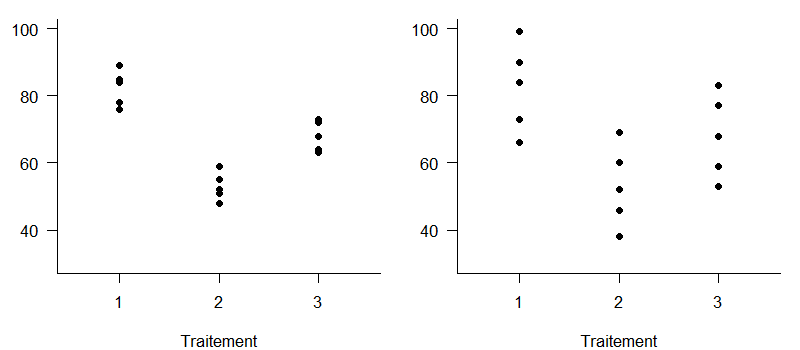
\includegraphics[width=10cm]{quiz1.png}
\vspace{1mm}

Quelle expérience a donné lieu au plus grand  $SS_{trt}$?\\au plus grand $SS_{E}$? au plus grand $SS_{T}$?
%\vspace{1cm}

\end{frame}
\begin{frame}[t]{ }

\centerline{\LARGE\bf \alert{QUIZ !}}
\medskip

{\small 2 expériences ont obtenu les mêmes variances échantillonnales:}

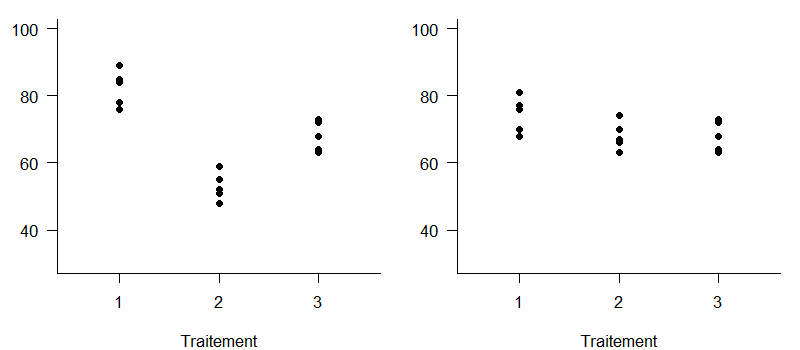
\includegraphics[width=10cm]{quiz2.png}
\vspace{1mm}

Quelle expérience a donné lieu au plus grand  $SS_{trt}$?\\ au plus grand $SS_{E}$? au plus grand $SS_{T}$?
%\vspace{1cm}

\end{frame}

\begin{frame}[t]{Statistique de test}

{\small
Pour déterminer si $SS_{trt}$ est suffisamment élevée par rapport à $SS_T$ pour rejeter $H_0$, on
utilise l'approche suivante.

On peut montrer que
\begin{itemize}\itemsep0.2cm
\item[$\bullet$]$\displaystyle\frac{SS_{trt}}{\sigma^2} \sim \chi_{\;a-1}^2~~ \mbox{si} ~~H_0~~\mbox{est vraie}$
\item[$\bullet$]%$\displaystyle\frac{SS_T}{\sigma^2} \sim \chi_{\;N-1}^2$, \hspace{1cm}
 $\displaystyle\frac{SS_E}{\sigma^2} \sim \chi_{\;an-a}^2$
\item[$\bullet$] $\dfrac{SS_{trt}}{\sigma^2}$ et $\dfrac{SS_{E}}{\sigma^2}$ sont indépendantes
\end{itemize}
 \vspace{0.3cm}

\medskip
On peut en déduire que si $H_0$ est vraie,
$$ F_0=\frac{SS_{trt}/(a-1)}{SS_E/(an-a)}\sim F_{a-1,\;an-a}. $$
}
\end{frame}

\begin{frame}[t]{Tableau d'analyse de la variance}
Les logiciels résument habituellement cette décomposition de la variabilité dans
un \alert{tableau d'analyse de la variance} (table ANOVA):

\bigskip



\begin{tabular}{cccccc}\hline
Source de & Somme des & Degrés de & Carré & $\quad F_0\quad $ & Valeur $p$ \\
variabilité & carrés & liberté & moyen & & \\ \hline
\\
Traitement & $SS_{trt}$ & $a-1$ & $MS_{trt}=\frac{SS_{trt}}{a-1}$ & $F_0=\frac{MS_{trt}}{MS_E}$ & {\scriptsize $P(F_{a-1,an-a}>F_0)$}
\\ \\ \\
Erreur & $SS_E$ & $an-a$ & $MS_E=\frac{SS_E}{an-a}$ & &
\\ \\ \\\hline \\
Totale & $SS_T$ & $an-1$ & & & \\ \\\hline
\end{tabular}


\end{frame}

\begin{frame}{Espérance des carrés moyens}
On peut montrer que
\vspace{0.3cm}

\begin{itemize}\itemsep1cm
\item[$\bullet$] $E(MS_{trt})=\sigma^2\;+\; \dfrac{n\sum\limits_{i=1}^a \tau_i^2}{a-1}$
\item[$\bullet$] $E(MS_{E})=\sigma^2$ $\rightarrow$ on se souvient que $MS_E$ est notre estimateur de $\sigma^2$
\item[$\bullet$] Si $H_0$ est vraie,
\item[$\bullet$] Si $H_1$ est vraie,
\end{itemize}
\vspace{1cm}

\end{frame}
%%%%%%%%%%%%%%%%%%%%%%%%%%%%%%%%%%%%%%%%%%%%%%%%%%%%%%%%%%%%%%%%%%%%%%%%%%%%%%%%%%%%%%%%%%%%%%%%%%%%%%%%%%%%%%%%%%%%%%%%%%%

\begin{frame}[t]{Exemple 2: inférence sur les résistances moyennes}

{\small
La force moyenne de résistance de la  fibre textile est-elle différente selon la proportion de coton, au seuil de 5\%? \\

\medskip
\begin{center}
\begin{tabular}{c|ccccc|rrr}\hline
Pourcentage & \multicolumn{5}{c|}{Observations $j$} & Somme & Moy.& É.-type\\
de coton $i$ & 1 & 2 & 3 & 4 & 5 & $y_{i\bullet}$ & $\overline{y}_{i\bullet}$ & $s_i$\\ \hline
15 & 7 & 7 & 15 & 11 & 9 & 49 & 9,8 &3,35\\[1mm]
20 & 12 & 17 & 12 & 18 & 18 & 77 & 15,4 &3,13\\[1mm]
25 & 14 & 18 & 18 & 19 & 19 & 88 & 17,6&2,07 \\[1mm]
30 & 19 & 25 & 22 & 19 & 23 & 108 & 21,6&2,61 \\[1mm]
35 & 7 & 10 & 11 & 15 & 11 & 54 & 10,8 &2,86\\ \hline
&&&&&&\multicolumn{2}{r}{$\overline{y}_{\bullet\bullet}=$15,04}
\end{tabular}
\end{center}
}

\vfill
{\tiny Source: {\it Design and Analysis of Experiments}, D.C. Montgomery (2001).}
\end{frame}


\begin{frame}[t]{Exemple 2 : pré-calculs pour la table d'anova }


\end{frame}

\begin{frame}[t]{Exemple 2 : table d'anova et seuil observé }


\begin{tabular}{cccccc}\hline
Source de & Somme des & Degrés de & Carré  & $\quad F_0 \quad$ & Valeur $p$ \\
variabilité & carrés & liberté & moyen & & \\ \hline
\\
Traitement & %$SS_{trt}$ & $a-1$ & $MS_{trt}=\frac{SS_{trt}}{a-1}$ & $F_0=\frac{MS_{trt}}{MS_E}$ & $P(F_{a-1,\{an-a\}}>F_0)$
\\ \\ \\
Erreur & %$SS_E$ & $an-a$ & $MS_E=\frac{SS_E}{an-a}$ & &
\\  \\\hline \\
Totale & %$SS_T$ & $an-1$ & & &
\\ \\ \hline
\end{tabular}

\end{frame}

\begin{frame}[t]{Exemple 2 : Décision et conclusion}

\underline{Décision}: $\qquad\square $ On rejette $H_0$ \hfill $\qquad\square $ On ne rejette pas $H_0$

\vspace{7mm}

\underline{Conclusion}: \\

\bigskip

Le pourcentage de coton $\left\{\begin{array}{c}\text{a un effet significatif}\\\text{n'a pas d'effet significatif}\end{array}\right\}$ \\

\medskip
sur la force moyenne de la fibre textile, au seuil de 5\%.
\end{frame}



\begin{frame}[t]{ }

\centerline{\LARGE\bf \alert{QUIZ !}}
\bigskip

Lorsque $H_0$ est rejetée, lesquelles des conclusions suivantes sont correctes?

\bigskip

\begin{enumerate}[$\square$]\itemsep 3mm
\item Toutes les moyennes sont égales.
%\item Toutes les variances sont égales.
\item Toutes les moyennes sont différentes.
\item Au moins deux moyennes sont différentes.
\item La variable réponse a un effet sur le facteur.
\item Le facteur a un effet sur la variable réponse.
\end{enumerate}

\vspace{3mm}


\end{frame}


\section{Validation des postulats}
\subsection*{ }
\begin{frame}[t]{Postulats à valider}
L'inférence (test $F$) est basée sur trois postulats:
\begin{itemize}
\item[(P1)] l'indépendance des observations;
\item[(P2)] l'homogénéité des variances d'un traitement à l'autre;
\item[(P3)] la normalité des $E_{ij}$.
\end{itemize}

(P2) et (P3) peuvent être validés graphiquement.\\

\uncover<2->{
Les erreurs $E_{ij}$ sont inconnues. On les estime avec les {\it résidus}.\\
%Or, on observe les $Y_{ij}$, et on sait estimer $\mu$ et les $\tau_i$.
}

\medskip
\uncover<3->{
\begin{Boite}{Résidus}
On estime  les $E_{ij}=Y_{ij}-\mu-\tau_i$ par les \alert{ résidus $e_{ij}$}:

$\begin{array}{ll}
\alert{e_{ij}}&=Y_{ij}-\hat{\mu}-\hat{\tau}_i\\
&=Y_{ij}-\overline{Y}_{\bullet\bullet}-(\overline{Y}_{i\bullet}-\overline{Y}_{\bullet\bullet})\\ &=\alert{Y_{ij}-\overline{Y}_{i\bullet}}
\end{array}$
\end{Boite}}
\end{frame}


\begin{frame}[t]{Propriétés des résidus}

{\small
%Les résidus sont des v.a. qui ont un \alert{comportement aléatoire proche de celui des $E_{ij}$}.
Pour valider les deux postulats, on peut regarder les graphiques suivants:
\begin{itemize}
\item[(P2)] \alert{Homogénéité des variances:}  \\
\begin{itemize}
\item juxtaposer les $a$ diagrammes en bo\^{\i}te des résidus, ou\\ tracer les résidus pour chaque traitement\\{\color{gray}{\it (la dispersion devrait être similaire)}};
\item graphique des $e_{ij}$ en fonction des {\em valeurs ajustées $\overline{y}_{i\bullet}$}\\ {\color{gray}{\it (la distribution des $e_{ij}$ ne devrait pas changer selon les $\overline{y}_{i\bullet}$).}}
\end{itemize}
\item[(P3)] \alert{Normalité des erreurs:}\\
\begin{itemize}
\item histogramme des $an$ résidus \\{\color{gray}{\it (on devrait observer une forme de cloche symétrique)}};
\item diagramme quantile-quantile des $an$ résidus.\\ {\color{gray}{\it (on devrait voir une ligne assez droite).}}
\end{itemize}
\end{itemize}
}
\end{frame}

\begin{frame}[t]{Exemple 3 : Analyse des résidus}

%{\it Voir R Commander ...}
\begin{center}
    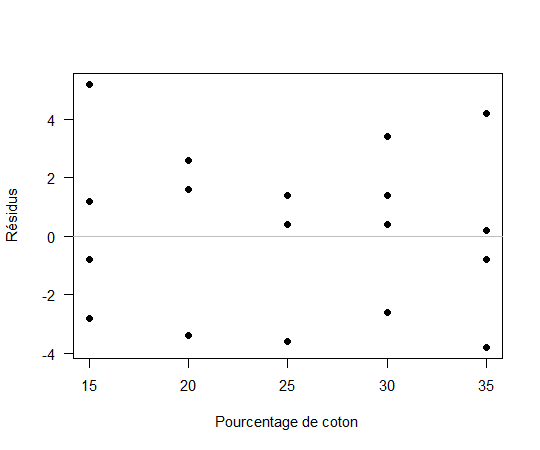
\includegraphics[scale=0.3]{res1b.png} \hspace{1cm}
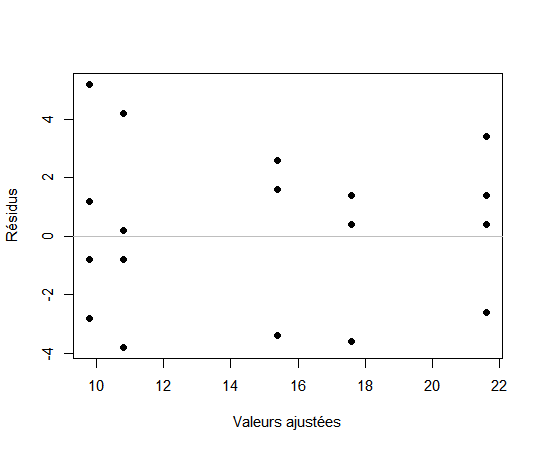
\includegraphics[scale=0.3]{res2.png}\\
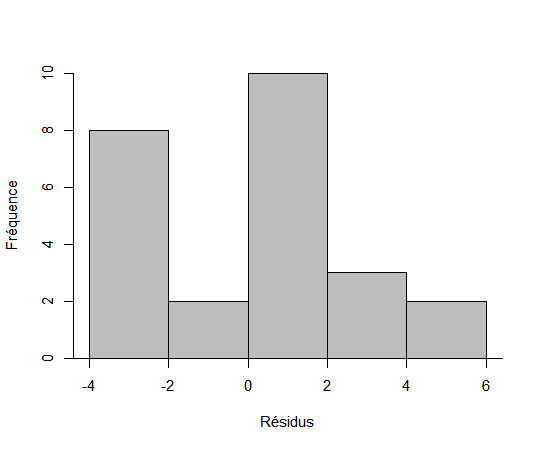
\includegraphics[scale=0.3]{res3.png} \hspace{1cm}
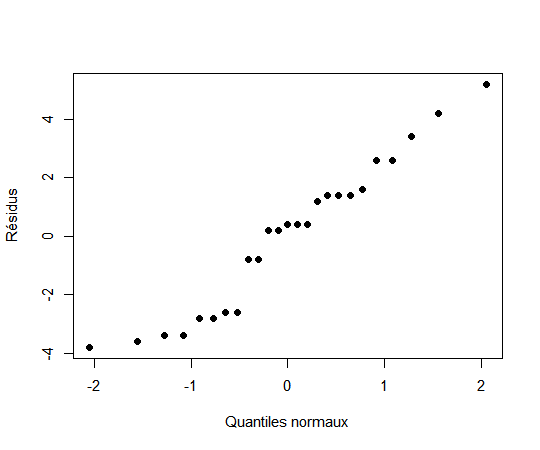
\includegraphics[scale=0.3]{res4.png}
\end{center}


\end{frame}

\begin{frame}[t]{Oui, mais...}

Que faire si les postulats ne semblent pas respectés, d'après l'analyse des résidus?

\medskip
\begin{itemize}\itemsep1.3cm
\item Tests de normalité (tests d'hypothèses non abordés dans le cours)
\item Transformation des $Y_{ij}$
\item Anova non paramétrique (test de Kruskall-Wallis, non abordé dans le cours)
\end{itemize}
\end{frame}


\section[Comparaisons 2 à 2]{Tests de comparaison des moyennes 2 à 2}\label{sec:ppds1fac}
\subsection*{ }

\begin{frame}[t]{Test $F$ significatif: la suite}

\begin{enumerate}
\item Si le test $F$ d'égalité des moyennes n'est pas significatif ($H_0$ non rejetée), l'analyse est terminée.
\vspace{.7cm}

\item Si le test global du tableau ANOVA nous mène à rejeter $H_0$, on veut savoir \underline{quelles} moyennes diff\`erent les unes des autres.
\vspace{.5cm}
\end{enumerate}

Plusieurs procédures permettent de faire les comparaisons de moyennes 2 \`a 2 (souvent appelées {\it tests de comparaisons multiples}).
\vspace{.5cm}

L'approche de la \alert{{\em plus petite différence significative} (PPDS)} de Fisher offre une réponse à cette question.
\end{frame}

\begin{frame}[t]{Approche ``PPDS'' de Fisher}

\begin{itemize}
\item On se base sur l'IC($\mu_i-\mu_k$) de niveau $1-\alpha$.
\item Si la différence entre les moyennes est supérieure à la marge d'erreur de cet intervalle (en valeur absolue), on les déclarera significativement différentes au seuil $\alpha$.

%\item $(\overline{Y_{i\bullet}}-\overline{Y_{k\bullet}})\pm$

\end{itemize}
\medskip
\uncover<2->{
\begin{Boite}{Approche PPDS de Fisher}
$$
PPDS=t_{\alpha/2;an-a}\sqrt{\dfrac{2MS_E}{n}}.
$$
On déclare \alert{significativement différentes au seuil $\alpha$} toute paire
de moyennes qui diffèrent (en val. abs.) par au moins PPDS.
\end{Boite}
}
\end{frame}

\begin{frame}[t]{Exemple 4: calcul de la $ PPDS$}

{\small
Nous avions conclu que les moyennes des 5 traitements n'étaient pas toutes égales. Mais quelles paires de moyennes sont significativement différentes au seuil de 5\%?}
\end{frame}

\begin{frame}[t]{Exemple 4 : comparaisons 2 à 2}

 $$
\begin{array}{c c c c c}
\;\;\;\;\overline y_{1\bullet} \;\;\;\;&\;\;\;\; \overline
y_{5\bullet} \;\;\;\;& \;\;\;\;\overline y_{2\bullet} \;\;\;\;
&\;\;\;\;\overline y_{3\bullet} \;\;\;\;&\;\;\;\;
\overline y_{4\bullet} \;\;\;\;\\[.3cm]
9,8 & 10,8 & 15,4 & 17,6 & 21,6\\[.3cm]
\textrm{\scriptsize 15\%}&
\textrm{\scriptsize 35\%}&
\textrm{\scriptsize 20\%}&
\textrm{\scriptsize 25\%}&
\textrm{\scriptsize 30\%}
\end{array}
$$
\end{frame}


\begin{frame}[t]{Réponses aux exemples}

{\scriptsize

\begin{enumerate}
  \item  $\hat\mu=\overline y_{\bullet\bullet}=15,04;\, \hat\tau_1=-5,24;\, \hat\tau_2=0,36;\, \hat\tau_3=2,56;\, \hat\tau_4=6,56;\, \hat\tau_5=-4,24;\,\hat\sigma^2=8,06$
 \item $\mbox{ }$

 \begin{tabular}{cccccc}\hline
Source de & Somme des & Degrés de & Carré & $\quad F_0\quad $ & Valeur $p$ \\
variabilité & carrés & liberté & moyen & & \\ \hline
Traitement & $475,8$ & $4$ & $118,91$ & $14,76$ & $9,13\times 10^{-6}$\\
Erreur & $161,2$ & $20$ &$ 8,06$ & & \\\hline
Totale &$637,0$ &$24$ & & & \\\hline
\end{tabular}

      Effet significatif du pourcentage de coton.
 \item Variances très similaires, normalité questionnable (bimodalité).
 \item $PPDS=3,75$
  $$
\begin{array}{c c c c c}
\;\;\;\;\overline y_{1\bullet} \;\;\;\;&\;\;\;\; \overline
y_{5\bullet} \;\;\;\;& \;\;\;\;\overline y_{2\bullet} \;\;\;\;
&\;\;\;\;\overline y_{3\bullet} \;\;\;\;&\;\;\;\;
\overline y_{4\bullet} \;\;\;\;\\[.3cm]
9,8 & 10,8 & 15,4 & 17,6 & 21,6
%\textrm{\scriptsize 15\%}& \textrm{\scriptsize 35\%}& \textrm{\scriptsize 20\%}& \textrm{\scriptsize 25\%}& \textrm{\scriptsize 30\%}
\\ \cline{1-2}\\\cline{3-4}
\end{array}
$$
 \end{enumerate}

 }
\end{frame}

\begin{frame}[t]{Adaptation de la méthode}

Comme plusieurs parmi vous le verrez dans un cours de troisième ou quatrième année,
le modèle d'analyse de la variance à un facteur peut être adapté/généralisé pour faire
face à des situations plus complexes. Par exemple :
\begin{itemize}
\item<1-> {\bf Contrôler la variabilité :} On peut généraliser le test t pour échantillons appariés
au cas où l'on a plus de 2 échantillons : plan d'expérience à blocs aléatoires
(voir section 11.2 du manuel du cours).
\item<2-> {\bf Étudier l'effet de plus d'un facteur :} On peut planifier des expériences servant
à étudier l'effet de plusieurs facteurs simultanément et en analyser les résultats à l'aide
d'une généralisation du principe de décomposition de la variance
(voir sections 11.3-11.4 du manuel du cours).
\end{itemize}

\end{frame}

\end{document}